%%%%%%%%%%%%%%%%%%%%%%%%%%%%%%%%%%%%%%%%%
% a0poster Portrait Poster
% LaTeX Template
% Version 1.0 (22/06/13)
%
% The a0poster class was created by:
% Gerlinde Kettl and Matthias Weiser (tex@kettl.de)
% 
% This template has been downloaded from:
% http://www.LaTeXTemplates.com
%
% License:
% CC BY-NC-SA 3.0 (http://creativecommons.org/licenses/by-nc-sa/3.0/)
%
%%%%%%%%%%%%%%%%%%%%%%%%%%%%%%%%%%%%%%%%%

%----------------------------------------------------------------------------------------
%	PACKAGES AND OTHER DOCUMENT CONFIGURATIONS
%----------------------------------------------------------------------------------------

\documentclass[a0,portrait]{a0poster}

\usepackage{multicol} % This is so we can have multiple columns of text side-by-side
\columnsep=100pt % This is the amount of white space between the columns in the poster
%\columnseprule=3pt % This is the thickness of the black line between the columns in the poster

\usepackage[svgnames,dvipsnames]{xcolor} % Specify colors by their 'svgnames', for a full list of all colors available see here: http://www.latextemplates.com/svgnames-colors

\usepackage{times} % Use the times font
%\usepackage{palatino} % Uncomment to use the Palatino font

\usepackage{graphicx} % Required for including images
\graphicspath{{figs/}} % Location of the graphics files
\usepackage{booktabs} % Top and bottom rules for table
\usepackage[font=small,labelfont=bf]{caption} % Required for specifying captions to tables and figures
\usepackage{amsfonts, amsmath, amsthm, amssymb} % For math fonts, symbols and environments
\usepackage{wrapfig} % Allows wrapping text around tables and figures
\usepackage{subcaption}
\usepackage{bm}
\usepackage{array}
\usepackage{amsmath,amssymb}
\usepackage{inconsolata}
\usepackage[T1]{fontenc}
\usepackage[scaled]{beramono}
\newcommand\Small{\fontsize{17}{19}\selectfont}
\newcommand*\LSTfont{\Small\ttfamily}
\usepackage{listings}
  \definecolor{mygreen}{rgb}{0,0.4,0}
  \lstset{
    language=LISP,
    comment=[l]{//},
    keywordstyle=\color{black},
    commentstyle=\color{mygreen},
    keywordstyle=[2]\color{RawSienna},
    keywords=[2]{assume,predict,infer,observe,DEFINE},
    keywordstyle=[3]\color{black},
    keywords=[3]{then,else,proc,tag,gamma,uniform_continuous,log,make_squaredexp,make_whitenoise,gpmem,mapv,first,repeat,do,mh,one,add_funcs,make_se,lambda,lookup,argmax_of_array,linspace,run,array,pass,mc_argmax,uniform_structure,subset,lte,if,flip,mult_funcs,for,to,get_neal_blackbox,get_neal_data_xs,get_data_xs,size,get_bayesopt_blackbox},
    basicstyle=\LSTfont,
    literate=%
    {0}{{{\color{DarkBlue}0}}}1
    {1}{{{\color{DarkBlue}1}}}1
    {2}{{{\color{DarkBlue}2}}}1
    {3}{{{\color{DarkBlue}3}}}1
    {4}{{{\color{DarkBlue}4}}}1
    {5}{{{\color{DarkBlue}5}}}1
    {6}{{{\color{DarkBlue}6}}}1
    {7}{{{\color{DarkBlue}7}}}1
    {8}{{{\color{DarkBlue}8}}}1
    {9}{{{\color{DarkBlue}9}}}1
  }



\newcommand{\gpmem}{\texttt{gpmem}}
\newcommand{\compute}{{\textrm{compute}}}
\newcommand{\emu}{{\textrm{emu}}}
\newcommand{\restr}{{\textrm{restr}}}
\newcommand{\true}{{\textrm{true}}}
\newcommand{\rmnew}{{\textrm{new}}}
\newcommand{\past}{{\textrm{past}}}
\newcommand{\prior}{{\textrm{prior}}}
\newcommand{\noisy}{{\textrm{noisy}}}
\newcommand{\noise}{{\textrm{noise}}}
\newcommand{\rmnext}{{\textrm{next}}}

\newcommand{\Acal}{\mathcal{A}}
\newcommand{\R}{\mathbb{R}}

\newcommand{\abf}{\mathbf{a}}
\newcommand{\fbf}{\mathbf{f}}
\newcommand{\rbf}{\mathbf{r}}
\newcommand{\wbf}{\mathbf{w}}
\newcommand{\xbf}{\mathbf{x}}
\newcommand{\ybf}{\mathbf{y}}
\newcommand{\Kbf}{\mathbf{K}}
\newcommand{\Ibf}{\mathbf{I}}

\newcommand{\pn}[1]{\left( #1 \right)}
\newcommand{\bkt}[1]{\left[ #1 \right]}
\newcommand{\br}[1]{\left\{ #1 \right\}}
\newcommand{\abs}[1]{\left\lvert #1 \right\rvert}
\newcommand{\Ebkt}[2][]{\mathbb{E}_{#1}\bkt{#2}}
\newcommand{\mvert}{\ \middle\vert\ }

\DeclareMathOperator*{\Cov}{Cov}
\DeclareMathOperator*{\argmax}{arg\,max}
\begin{document}

%----------------------------------------------------------------------------------------
%	POSTER HEADER 
%----------------------------------------------------------------------------------------

% The header is divided into two boxes:
% The first is 75% wide and houses the title, subtitle, names, university/organization and contact information
% The second is 25% wide and houses a logo for your university/organization or a photo of you
% The widths of these boxes can be easily edited to accommodate your content as you see fit
\begin{flushright}
\begin{minipage}[b]{0.25\linewidth}

\includegraphics[width=7cm]{mitlogo.png}
\hspace{1cm}

\includegraphics[width=8cm]{royalhollowaylogo.jpg}
\end{minipage} 
\end{flushright}

\vspace{2cm}

\begin{center}
\addtolength{\tabcolsep}{5pt} 
\veryHuge \textbf{Probabilistic Programming with Gaussian Process Memoization} \color{Black}\\[1.5cm] % Title
 \large   \begin{tabular}{  c  c  c c c}
           \textbf{Ulrich Schaechtle}  & \textbf{Ben Zinberg} & \textbf{Alexey Radul} & \textbf{Kostas Stathis}& \textbf{Vikash K. Mansinghka}\\ 
           Department of Computer Science & Computer Science \& AI Lab & Computer Science \& AI Lab & Department of Computer Science & Computer Science \& AI Lab \\
           Royal Holloway, Univ. of London & Massachusetts Institute of Technology & Massachusetts Institute of Technology & Royal Holloway, Univ. of London & Massachusetts Institute of Technology \\
        \end{tabular}

\addtolength{\tabcolsep}{-2pt} 
\end{center}



\vspace{3cm} % A bit of extra whitespace between the header and poster content

%----------------------------------------------------------------------------------------

\begin{multicols}{3} % This is how many columns your poster will be broken into, a portrait poster is generally split into 2 columns

%----------------------------------------------------------------------------------------
%	ABSTRACT
%----------------------------------------------------------------------------------------

%\color{Navy} % Navy color for the abstract

\begin{abstract}
This paper describes the {\em Gaussian process memoizer}, a probabilistic programming technique that uses Gaussian processes to provides a statistical alternative to memorization. Memoizing a target procedure results in a ``self-caching'' wrapper that remembers previously computed values. Gaussian process memoization additionally produces a statistical emulator based on a Gaussian process whose predictions automatically improve whenever a new value of the target procedure becomes available. This paper also introduces  an efficient implementation, named {\tt gpmem}, that can use kernels given by a broad class of probabilistic programs. The flexibility of {\tt gpmem} is illustrated via three applications: (i) GP regression with hierarchical hyper-parameter learning, (ii) Bayesian structure learning via compositional kernels generated by a probabilistic grammar, and (iii) a bandit formulation of Bayesian optimization with automatic inference and action selection. All applications share a single 85-line Python library and require fewer than 20 lines of probabilistic code each.
\end{abstract}


\color{DarkSlateGray} % DarkSlateGray color for the rest of the content
%\color{SaddleBrown} % SaddleBrown color for the introduction
%----------------------------------------------------------------------------------------
%	GP Memoization
%----------------------------------------------------------------------------------------
\section*{GP Memoization: \texttt{gpmem}}
\subsection*{Gaussian Processes}
$f(\xbf)$ is the multivariate Gaussian $f(\xbf) \sim \mathcal{N}(0, k(\xbf,\xbf))$,
where $k(\xbf,\xbf') = \Cov_f\pn{f(\xbf), f(\xbf')}$ is the covariance function, a.k.a.\ kernel.
The marginal likelihood can be expressed as:
\begin{equation*}
\label{eq:marg}
p\pn{f(\xbf) = \ybf \mvert \xbf} = \int p\pn{f(\xbf) = \ybf \mvert f, \xbf}\, p(f|\xbf) \, df
\end{equation*}


\subsection*{A Variation on Memoization}
{\em GP memoization} produces two components:
\[ f \to (f_\compute, f_\emu) \]
\begin{itemize}
\setlength{\itemindent}{1cm}
 \item is a generalization of traditional memoization;
 \item changes semantics of a probabilistic program;
 \item $f_\emu$ is a statistical emulator with GP prior;
 \item each time $f_\compute$ is called, an observation is incorporated into $f_\emu$ and predictions improve.
\end{itemize}


---------------------------------------------------------------------


%----------------------------------------------------------------------------------------
%	Bayesian GP
%----------------------------------------------------------------------------------------
\section*{Bayesian GP}

We show how we can use  {\tt gpmem} to reproduce Neal's Hierarchical Bayesian GP regression~\cite{neal1997monte} for data with outliers.

\begin{center}
Regression on data set $D$ \\
$\Updownarrow$ \\
Statistical emulation of $f_\restr(x) = \begin{cases}
      D[x], & \text{if $x$ is a data point} \\
      \text{Error}, & \text{otherwise}
    \end{cases}$
\end{center}
\vspace{1cm}
\begin{minipage}{\linewidth}
\belowcaptionskip=-10pt
\begin{lstlisting}[frame=single,mathescape,label=alg:gphierarch]
/// SETTING UP THE MODEL
assume alpha_sf = tag('hyperhyper, gamma(7, 1))
assume beta_sf = tag('hyperhyper, gamma(7, 1))
assume alpha_l = tag('hyperhyper, gamma(7, 1))
assume beta_l = tag('hyperhyper, gamma(7, 1))
// Parameters of the covariance function
assume log_sf = tag('hyper, log(gamma(alpha_sf, beta_sf))))
assume log_l = tag('hyper, log(gamma(alpha_l, beta_l))))
assume log_sigma = tag('hyper, log(uniform_continuous(0, 2)))

// The covariance function
assume se = make_squaredexp(sf, l)
assume wn = make_whitenoise(sigma)
assume composite_covariance = add_funcs(se, wn)

/// PERFORMING INFERENCE
// Create a prober and emulator using gpmem
assume f_restr = get_neal_blackbox()
assume compute_and_emu = gpmem(f_restr, composite_covariance)

// Probe all data points
predict mapv(first(compute_and_emu), get_neal_data_xs())

// Infer hypers and hyperhypers
infer repeat(100, do(
    mh('hyperhyper, one, 2),
    mh('hyper, one, 1)))

\end{lstlisting}
\end{minipage}
\subsection*{Results}
Ran the above program on data with outliers: noise $\sigma = 1.0$ with probability $0.05$, noise $\sigma = 0.1$ otherwise.
\begin{center}
\begin{tabular}{ccc}
  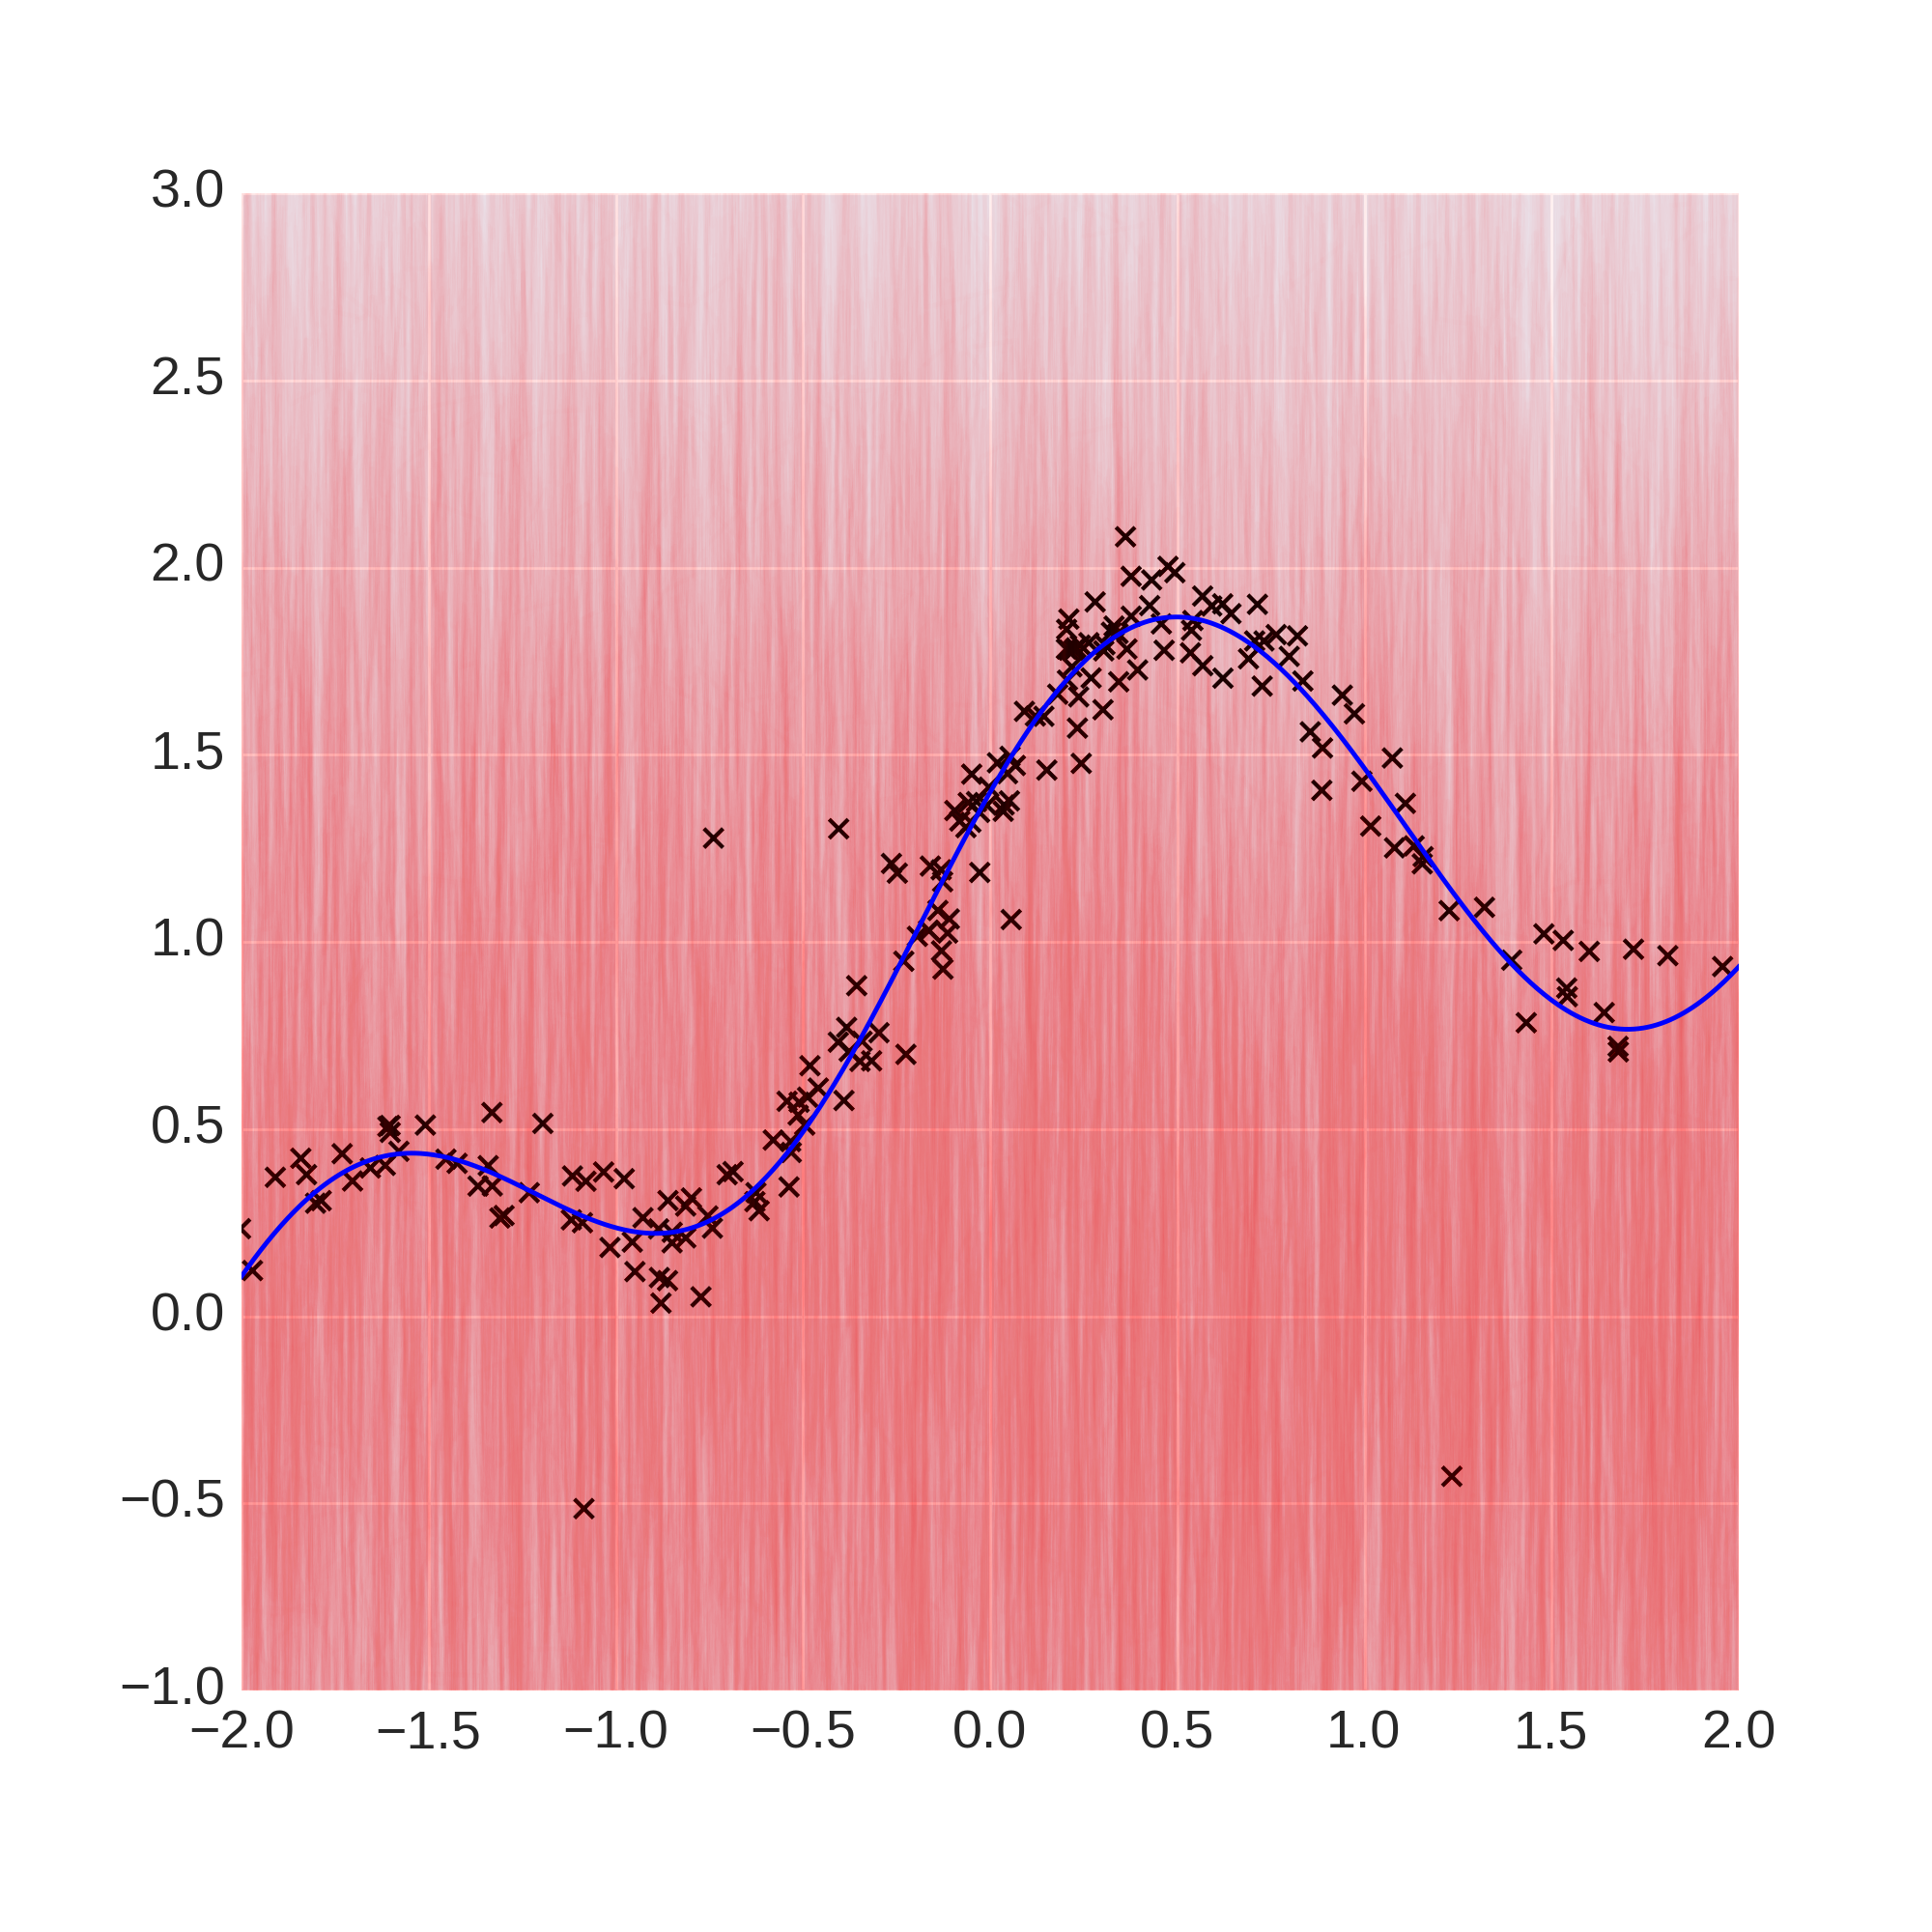
\includegraphics[width=8cm]{neal_se_1final.png}&
  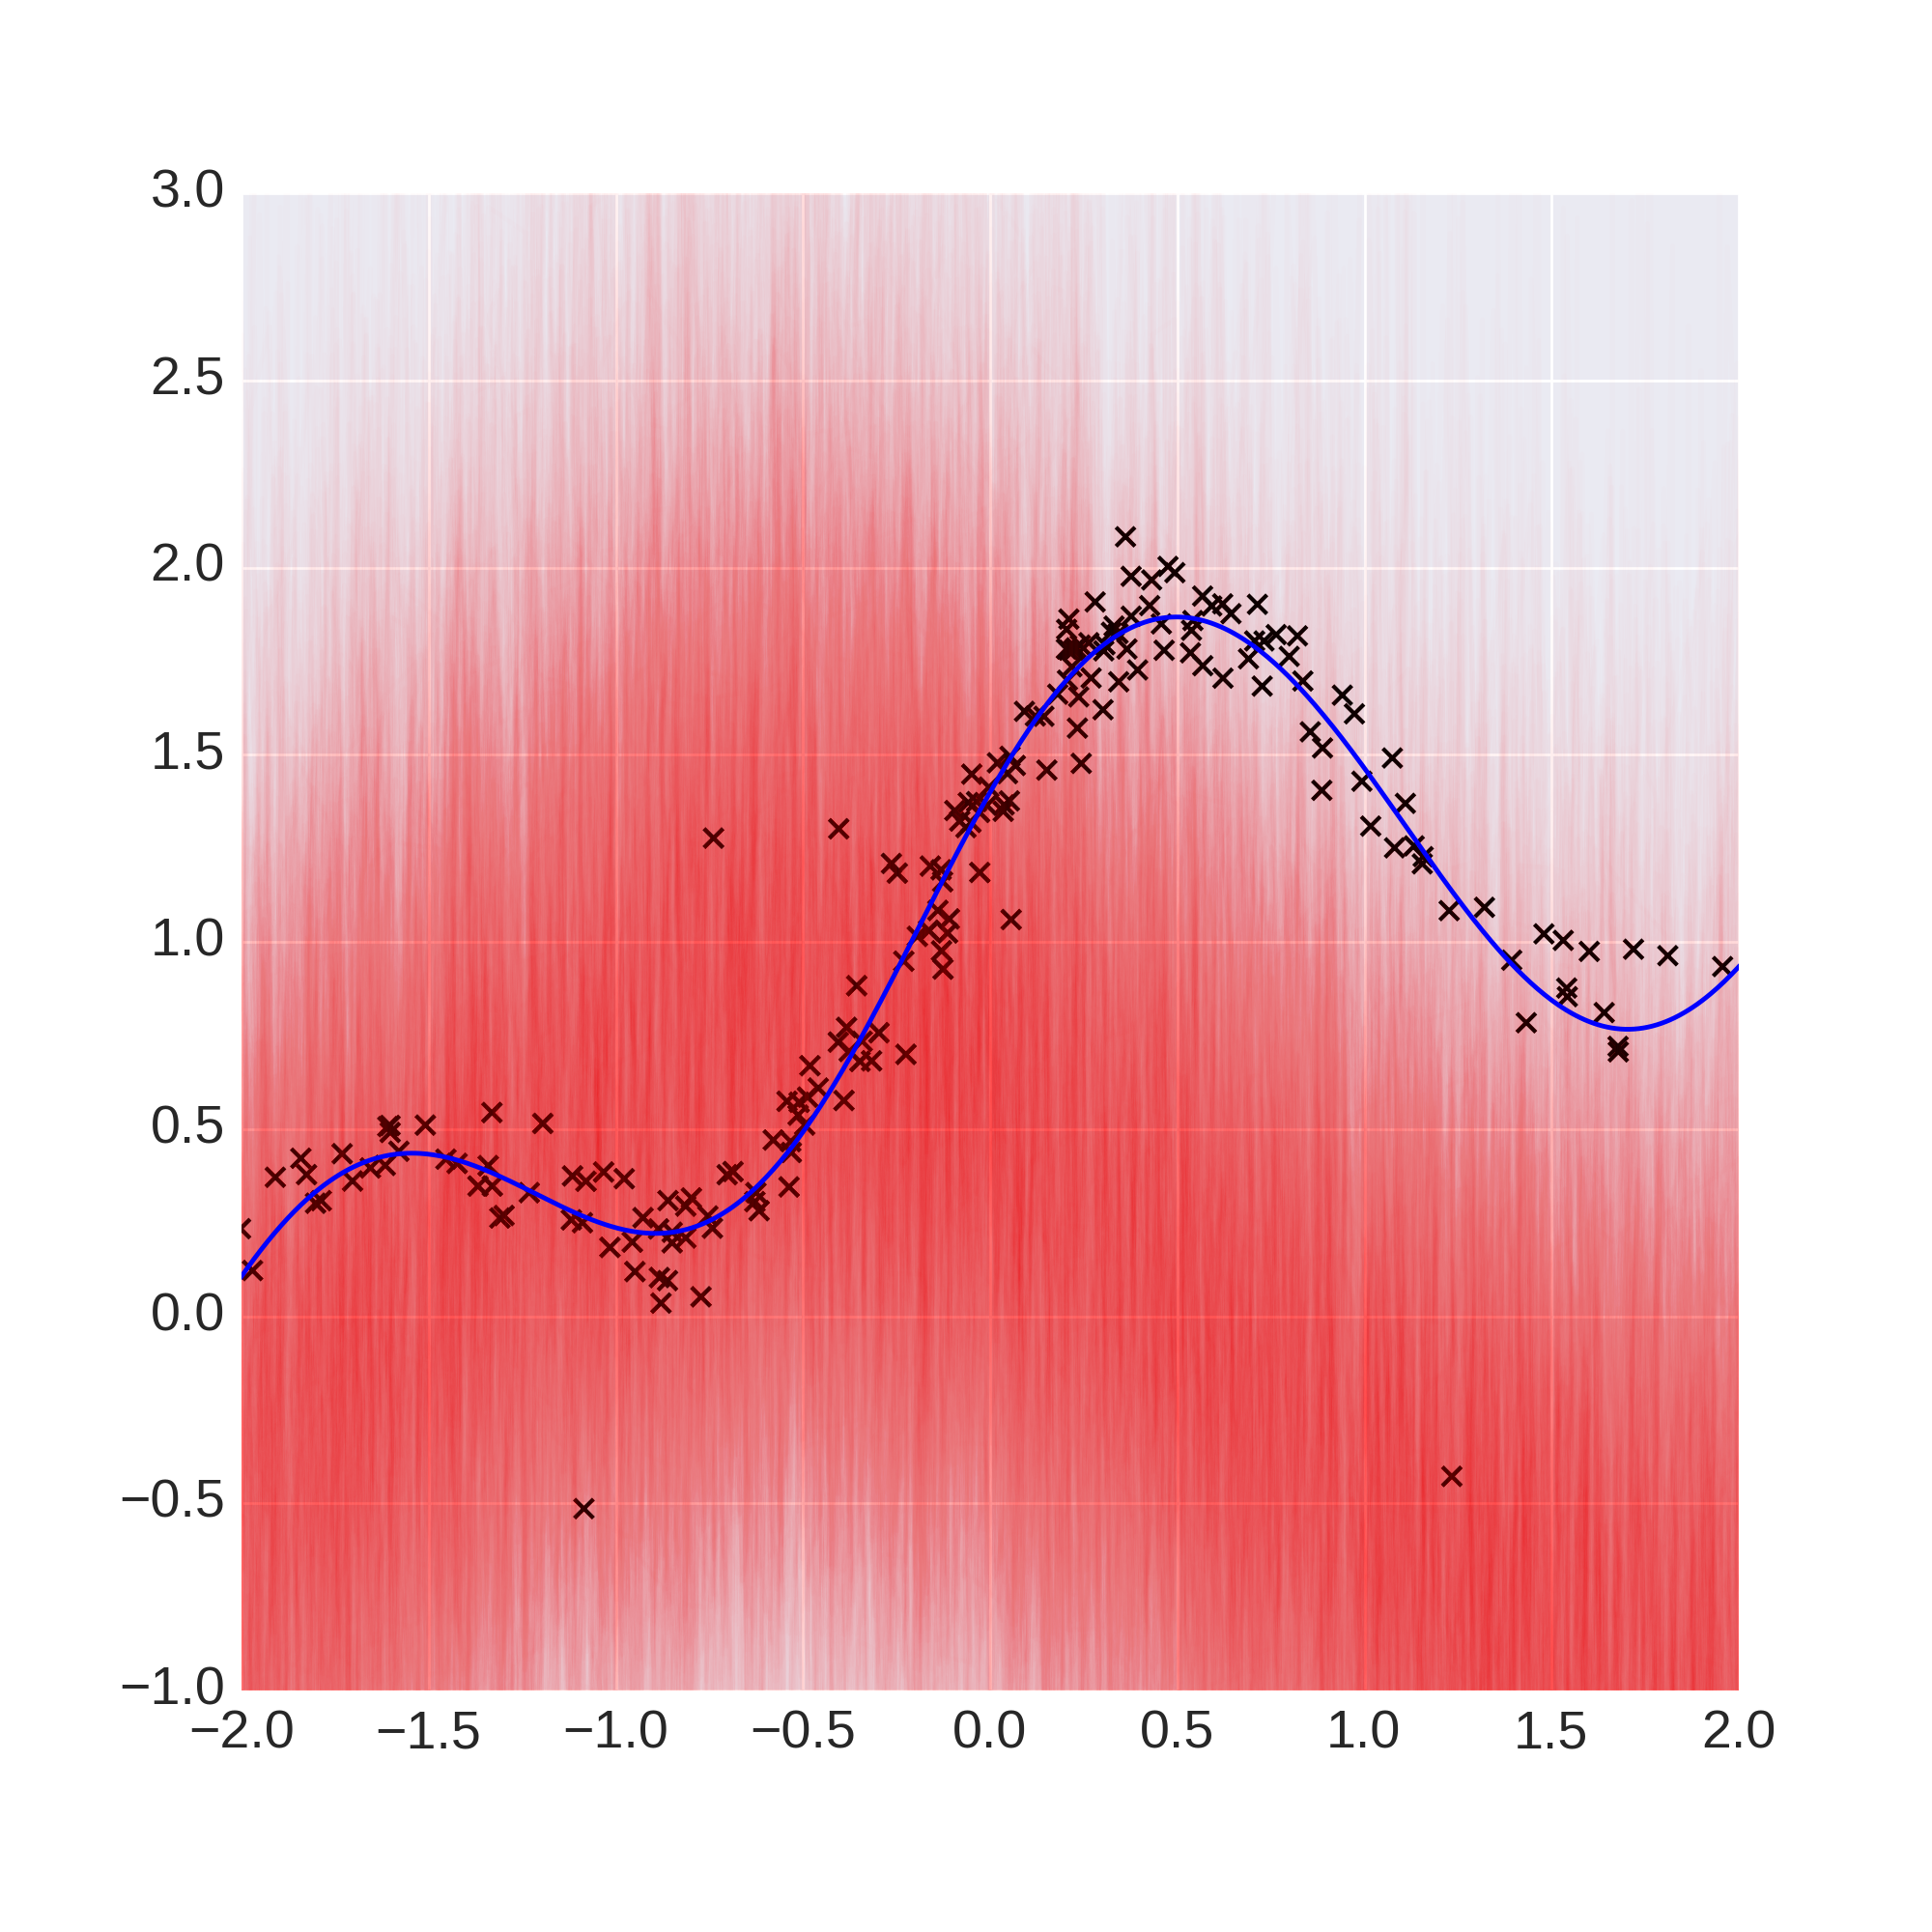
\includegraphics[width=8cm]{neal_se_2final.png}&
  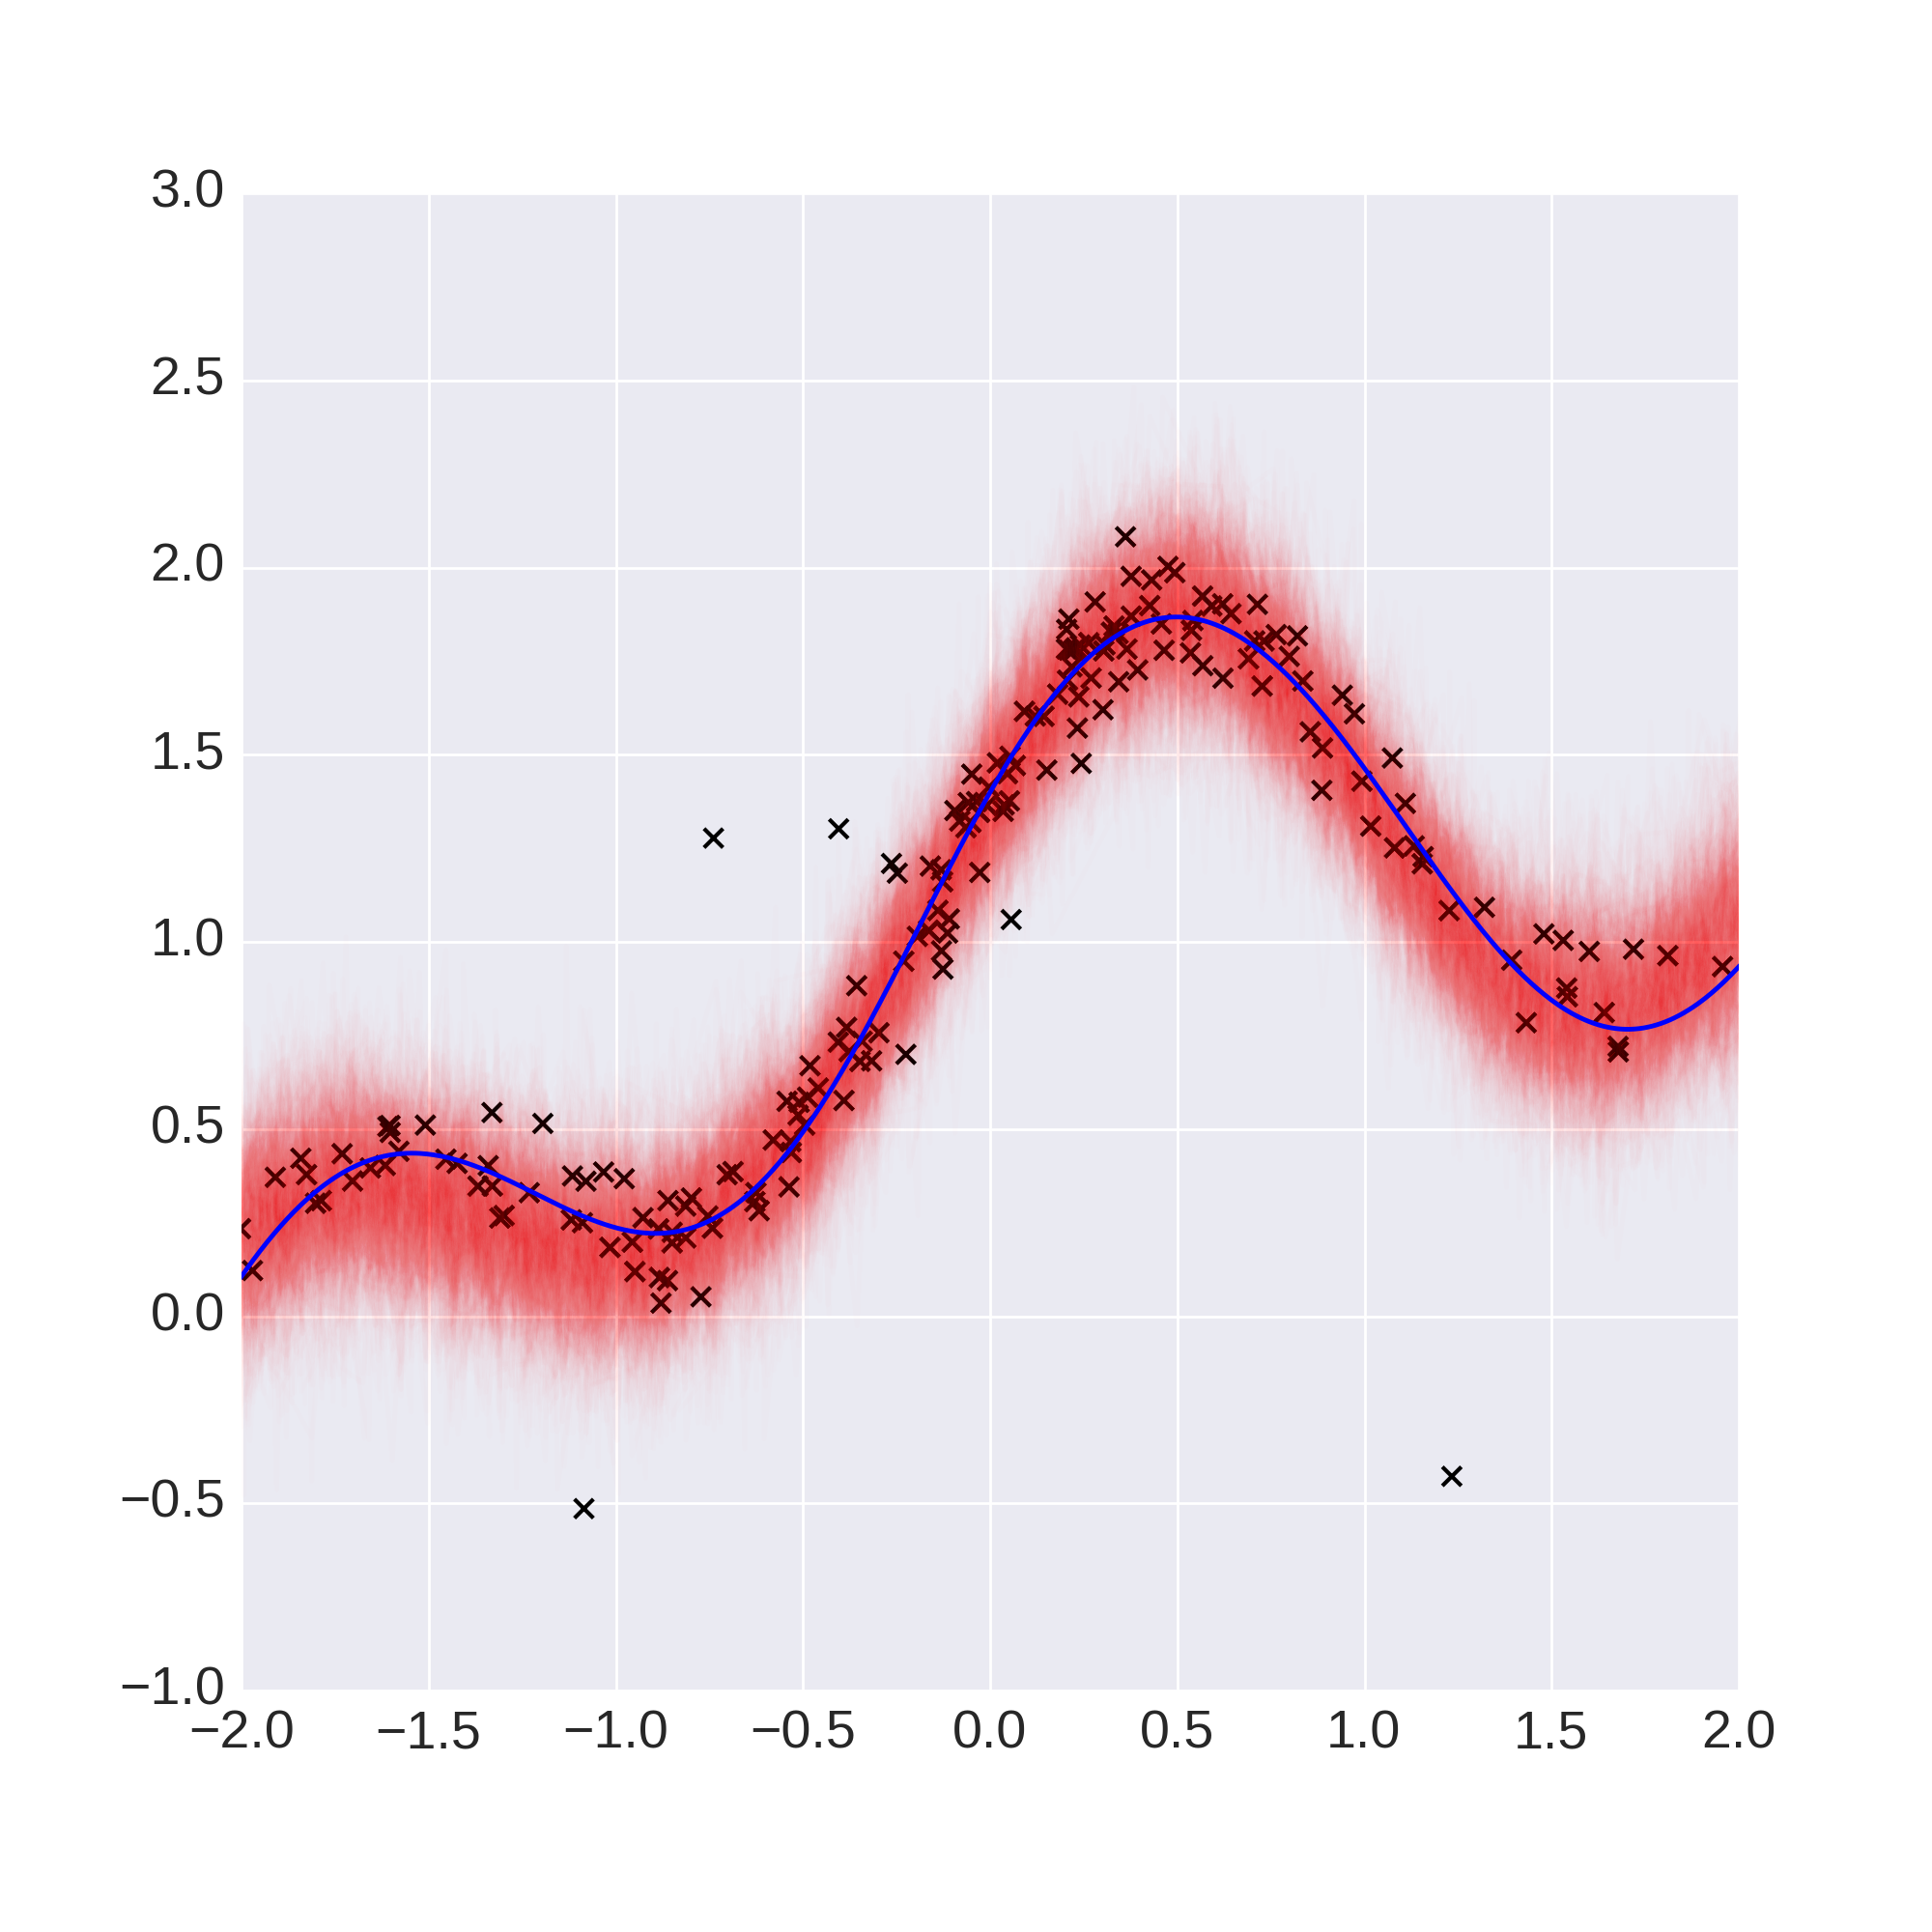
\includegraphics[width=8cm]{neal_se_3final.png}\\
  Data unobserved &
  Data observed &
  Hyperparameters inferred
\end{tabular}
\end{center}



%%\begin{wraptable}{r}{15cm} 
%\begin{center}
%%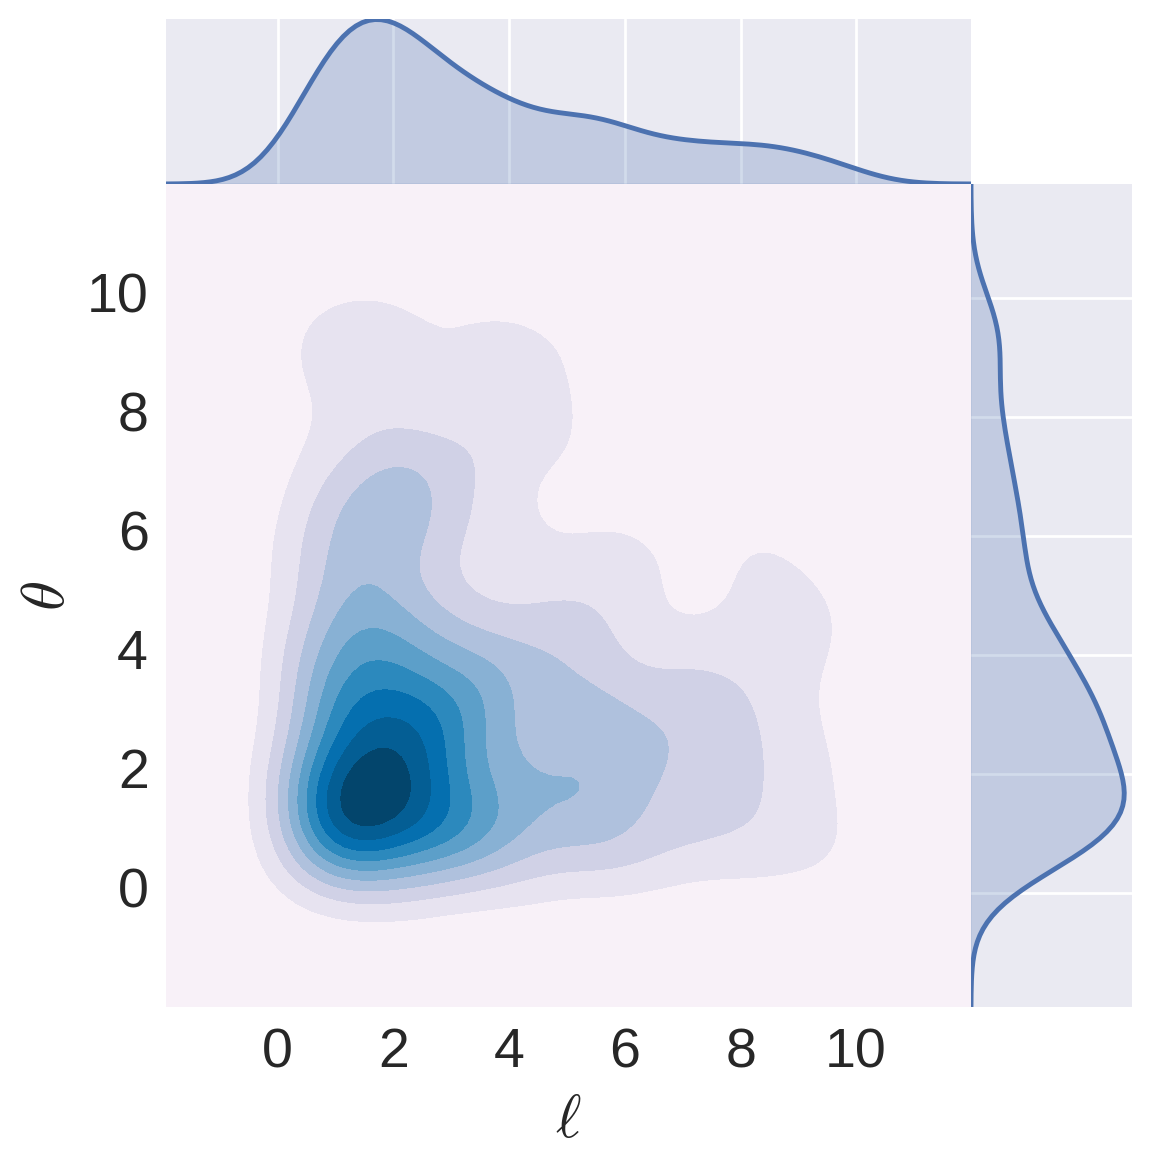
\includegraphics[width=10cm]{neal_contour_l_vs_sf_s__marginal_before.png}
%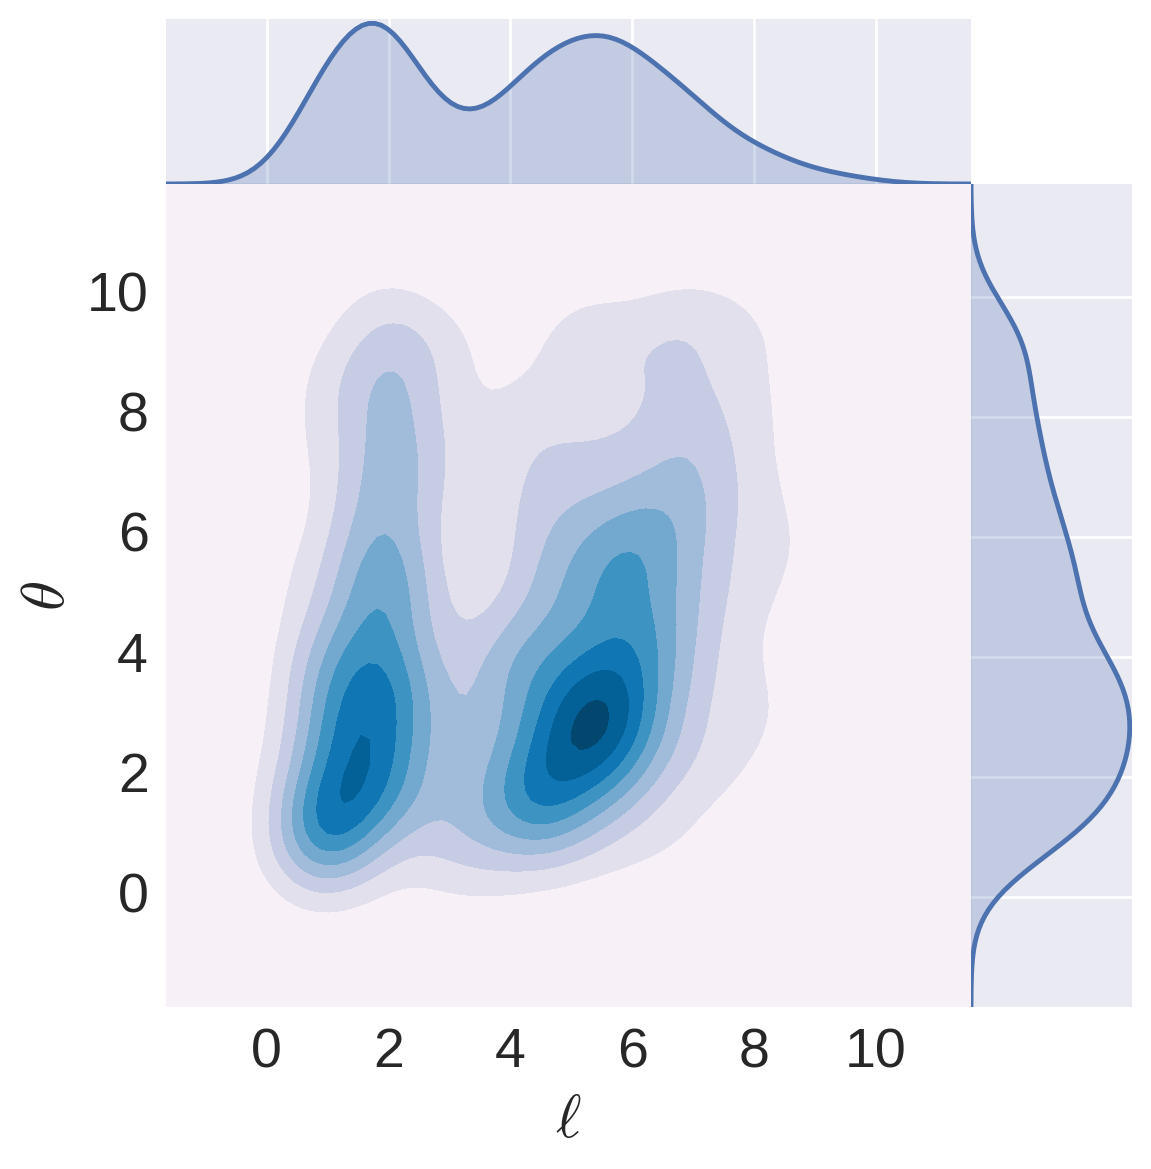
\includegraphics[width=7cm]{neal_contour_l_vs_sf_s__marginal_after.png} 
%\captionof{figure}{\color{DarkSlateGray}  Contour plot and marginals of the the l and sf hyper-parameters of the above program after inference}
%\end{center}
%
%\vfill
%\columnbreak


%----------------------------------------------------------------------------------------
%	Learning of Symbolic Structure
%----------------------------------------------------------------------------------------
\section*{GP Structure Learning}

\subsection*{Base Kernels}
 \begin{center} 
\begin{tabular}{m{11.5cm} m{4cm}}
$SE = \sigma^2 \exp(-\frac{(x-x^\prime)^2}{2\ell^2})$&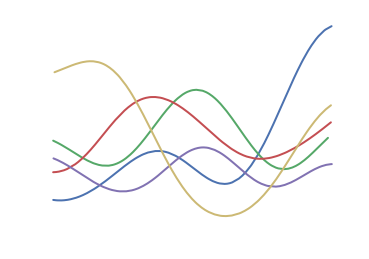
\includegraphics[width=4cm]{gpSamples/se.png}\\
$LIN = \theta (x x^\prime)$&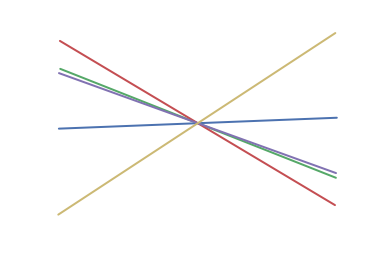
\includegraphics[width=4cm]{gpSamples/lin.png}\\
$PER = \theta \exp \bigg( \frac{2 \sin^2 ( \pi (x - x^\prime)/p}{\ell^2} \bigg)$&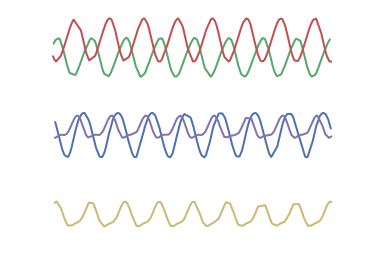
\includegraphics[width=4cm]{gpSamples/per.png}\\
$RQ =   \theta \bigg(1 + \frac{(x - x^\prime)^2}{2 \alpha \ell^2} \bigg)^{-\alpha}$&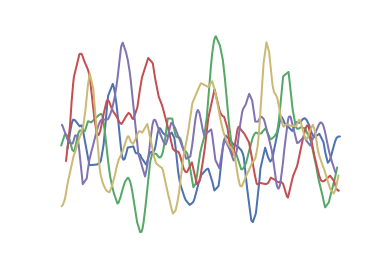
\includegraphics[width=4cm]{gpSamples/rq.png}
\end{tabular}
\end{center}
\subsection*{Kernel Composition}
\begin{equation*}
\mathbf{K}_{\textrm{new}} = \mathbf{K}_1 + \mathbf{K}_2 \;\;\;\;\;\;\text{or}\;\;\;\;\;\; \mathbf{K}_{\textrm{new}} = \mathbf{K}_1 \times \mathbf{K}_2 
\end{equation*}

\begin{center}\vspace{1cm}
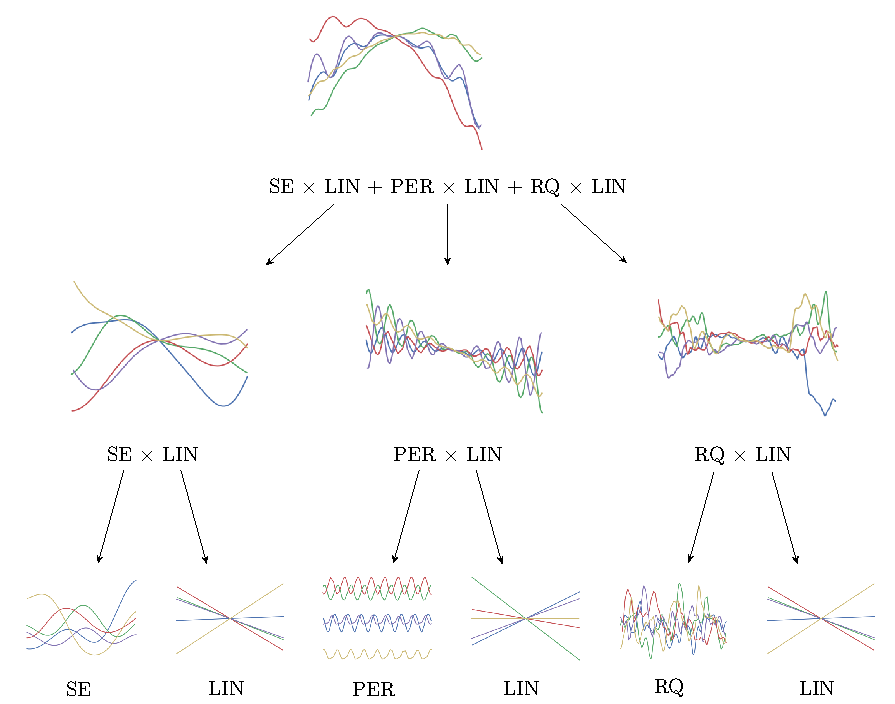
\includegraphics[width=0.8\linewidth]{parseTree.pdf}
%\captionof{figure}{\color{DarkSlateGray} Composition of covariance function parsed using the example SE $\times$ LIN $+$ PER $\times$ LIN $+$  RQ $\times$ LIN}
\end{center}
\vspace{1cm}

\begin{minipage}{\linewidth}
\small
\begin{lstlisting}[frame=single,label=alg:structureVent,mathescape]
// GRAMMAR FOR KERNEL STRUCTURE
assume base_kernels = list(se, wn, lin, per, rq) // defined as above

// prior on the number of kernels
assume p_number_k = tag('number_kernels, uniform_structure(n))
assume s = tag('choice_subset, subset(base_kernels, p_number_k))

assume cov_compo = proc(l) {
  // kernel composition
  if (size(l) <= 1)
  then { first(l) }
  else { if (flip()) then { add_funcs(first(l), cov_compo(rest(l))) }
                     else { mult_funcs(first(l), cov_compo(rest(l))) }
       }
  })
                          
assume K = tag('composit, cov_compo(s))

assume (f_compute f_emu) = gpmem(f_restr, K)
predict mapv(f_compute(get_data_xs)) // probe all data points

// PERFORMING INFERENCE  
infer  repeat(2000, do(
                        mh('number_kernel, one, 1),
                        mh('choice_subset, one, 1),
                        mh('composit, one, 1),
                        mh('hyper, one, 10)))
\end{lstlisting}

\end{minipage}



 
 \subsection*{Results}
 500 samples drawn from the posterior on structure for the CO2 dataset used in the Automated Statistician Project~\cite{duvenaud2013structure}:
 \begin{center}\vspace{1cm}
%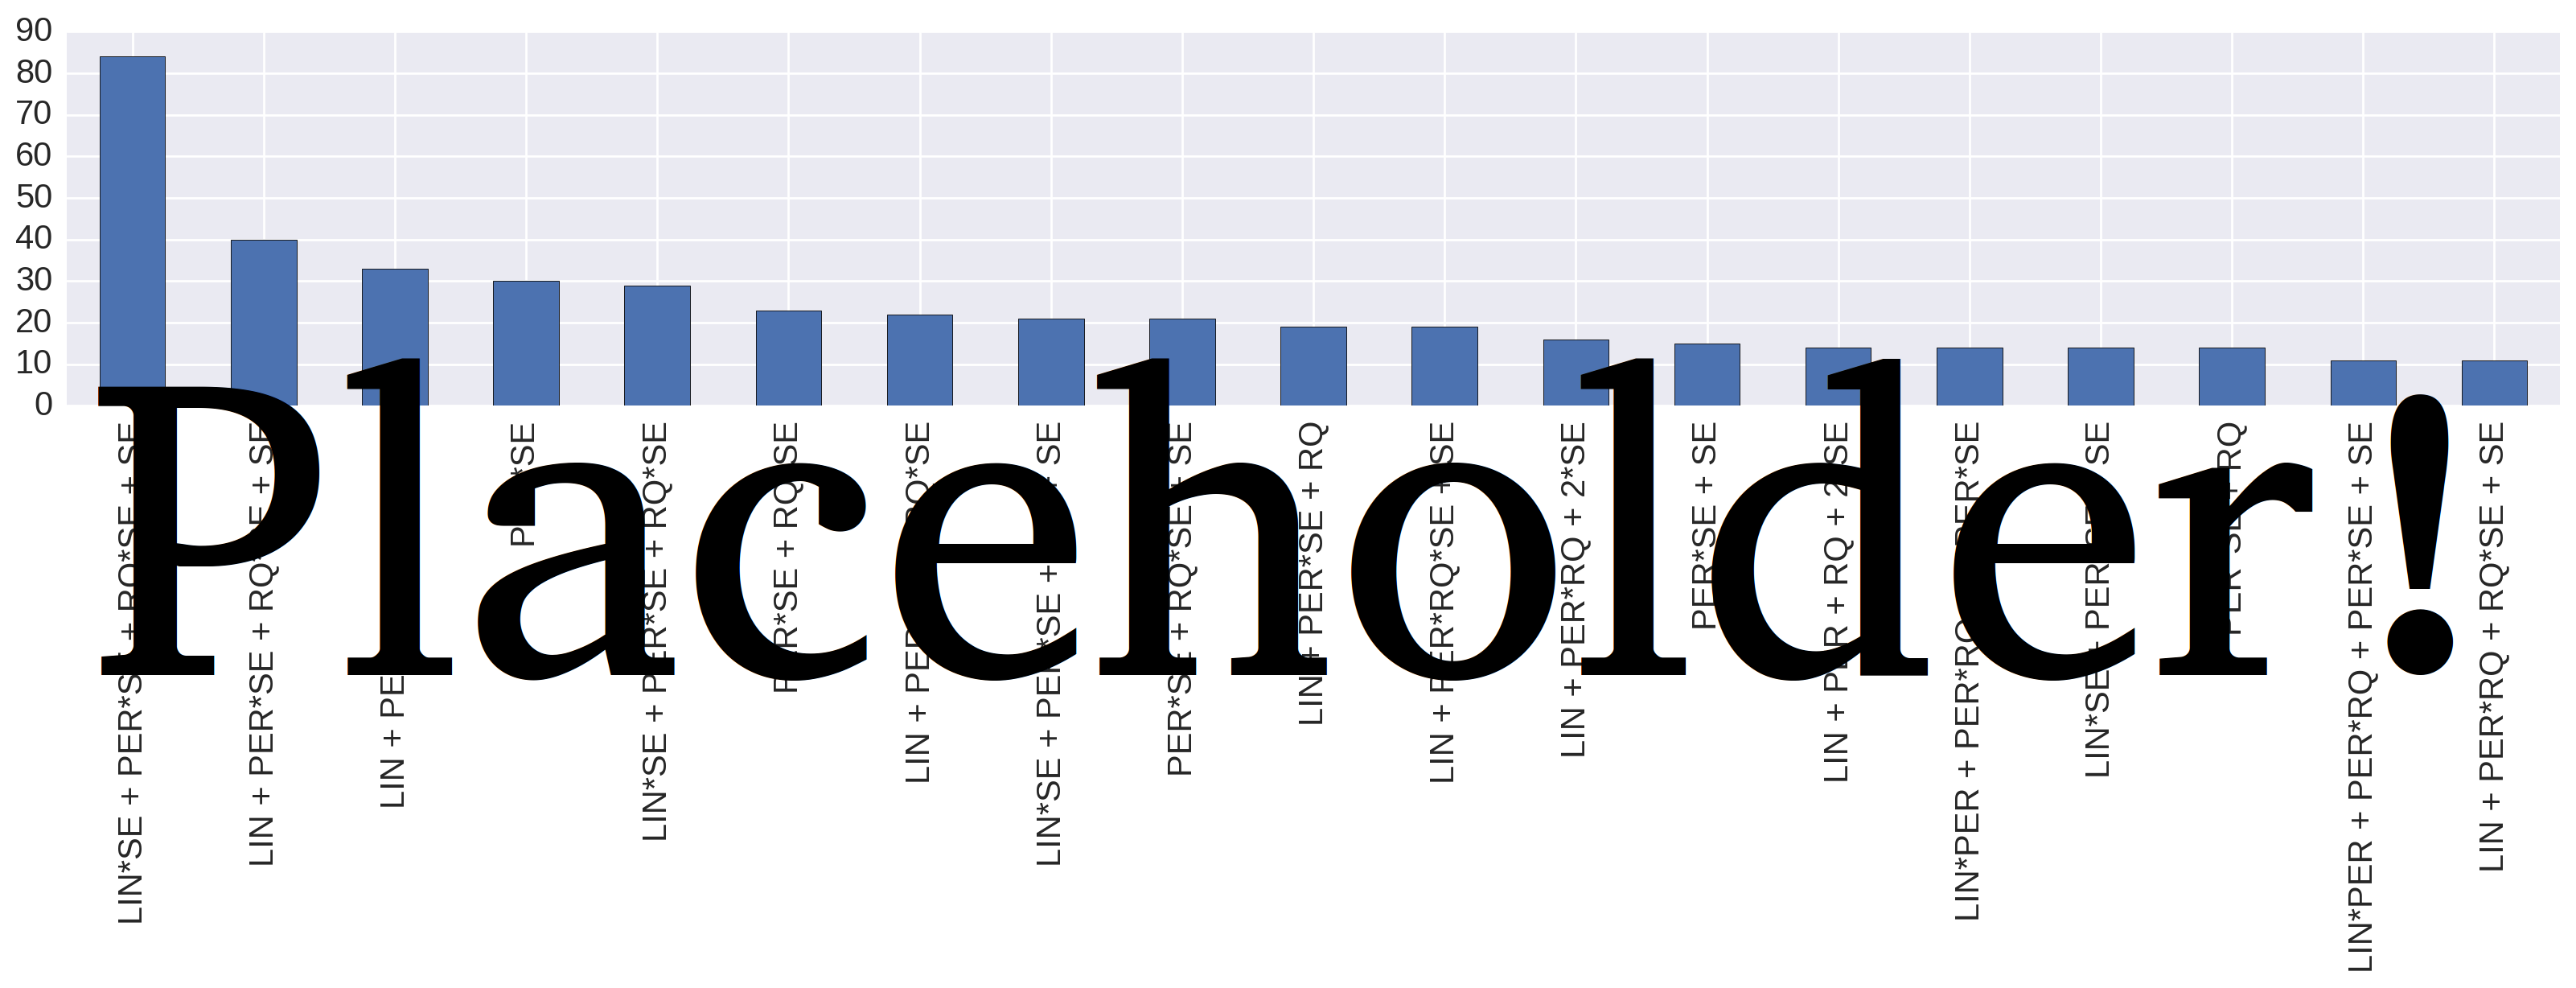
\includegraphics[width=0.7\linewidth]{structureCo2b.png}
%\captionof{figure}{\color{DarkSlateGray} Composition of covariance function parsed using the example SE $\times$ LIN $+$ PER $\times$ LIN $+$  RQ $\times$ LIN}
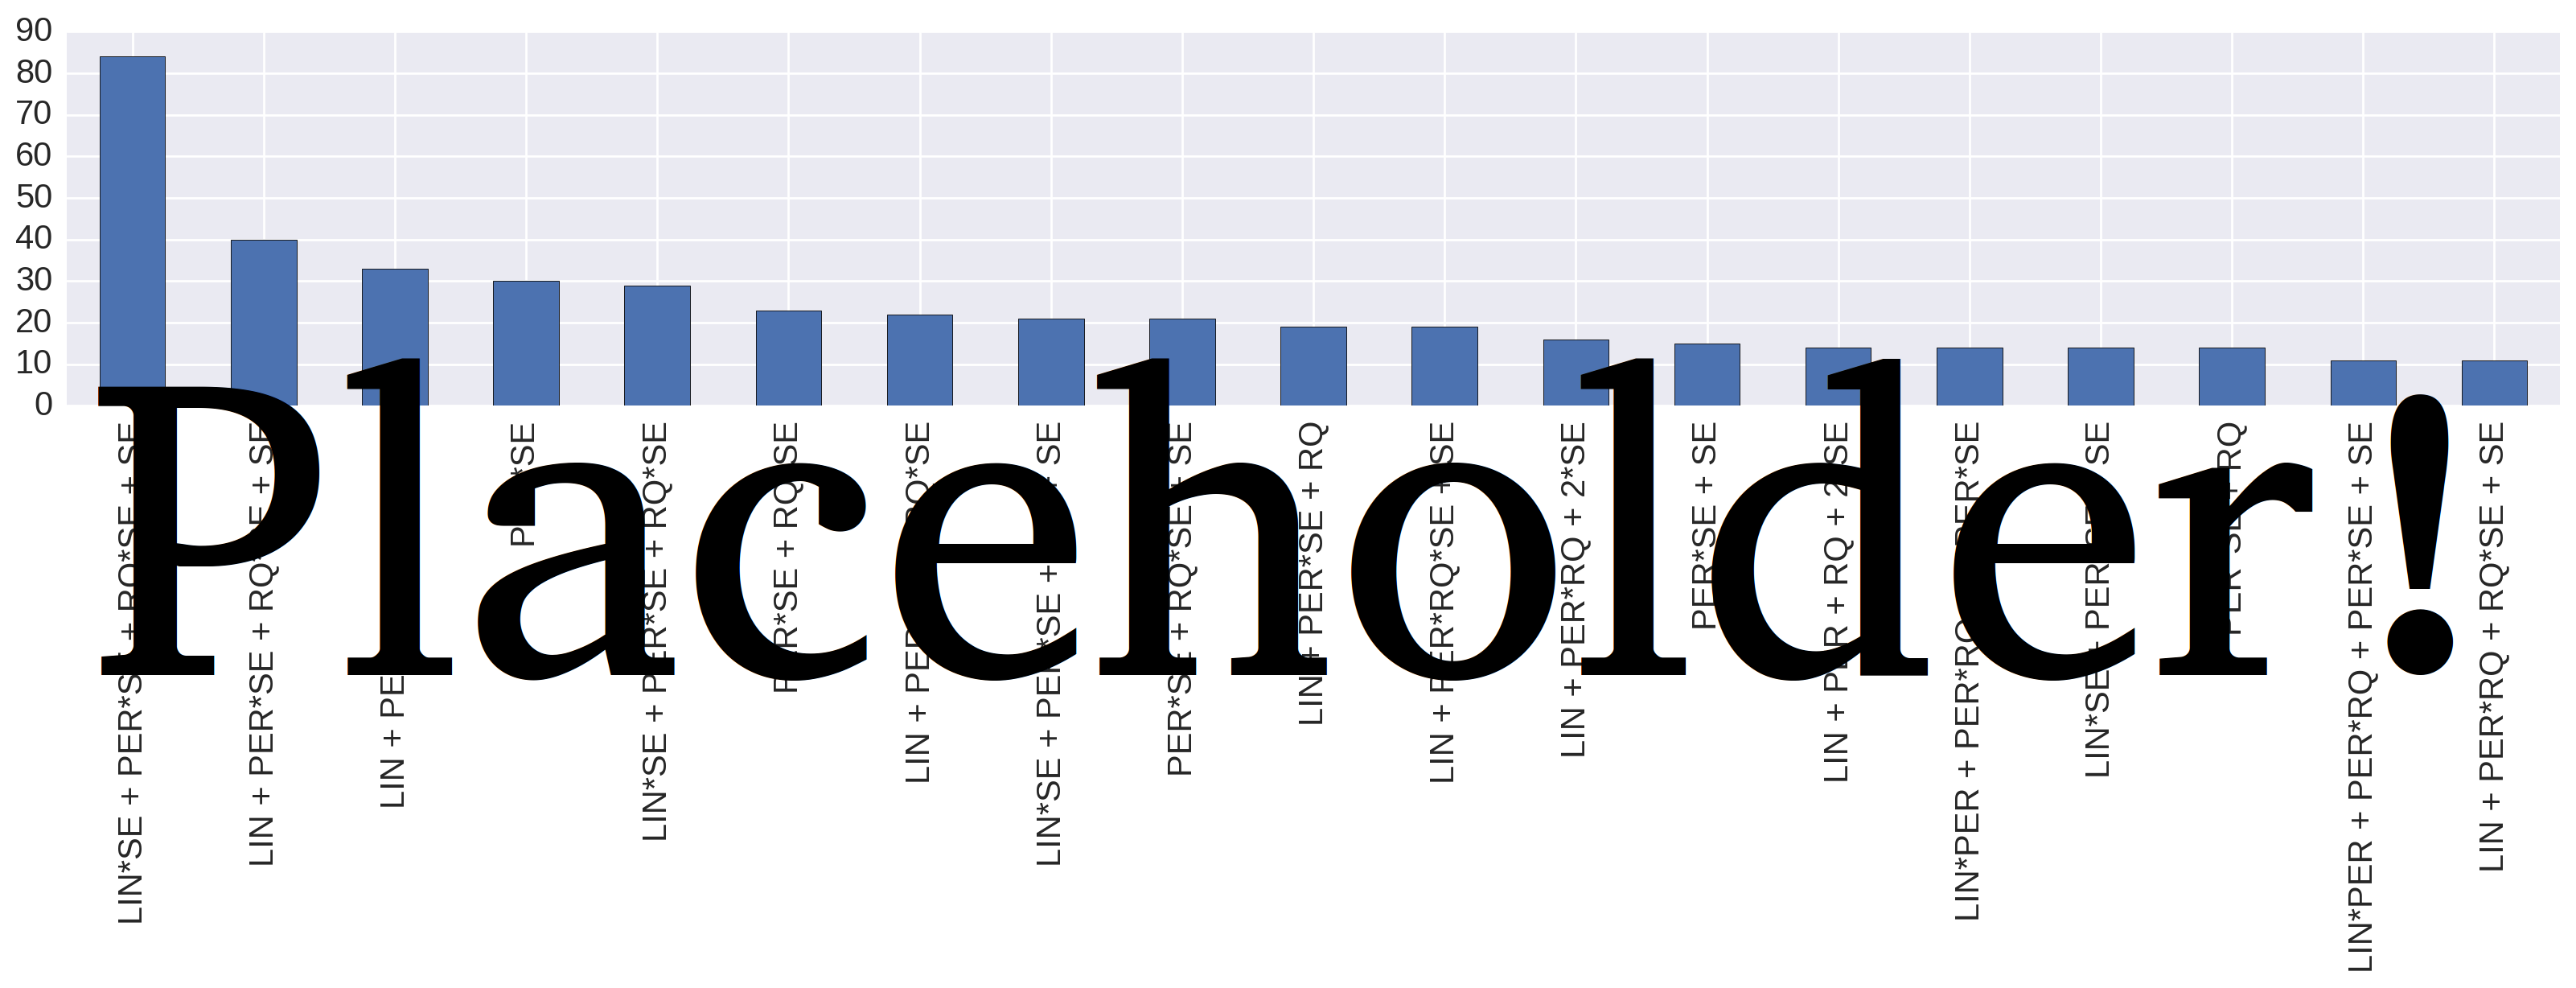
\includegraphics[width=0.7\linewidth]{structureCo2b.png}
\end{center}\vspace{1cm}
Posterior samples for curves for the airline dataset where SE $\times$ LIN $+$ PER $\times$ LIN $+$  RQ $\times$ LIN is sampled from the structure grammar:
 \begin{center}\vspace{1cm}
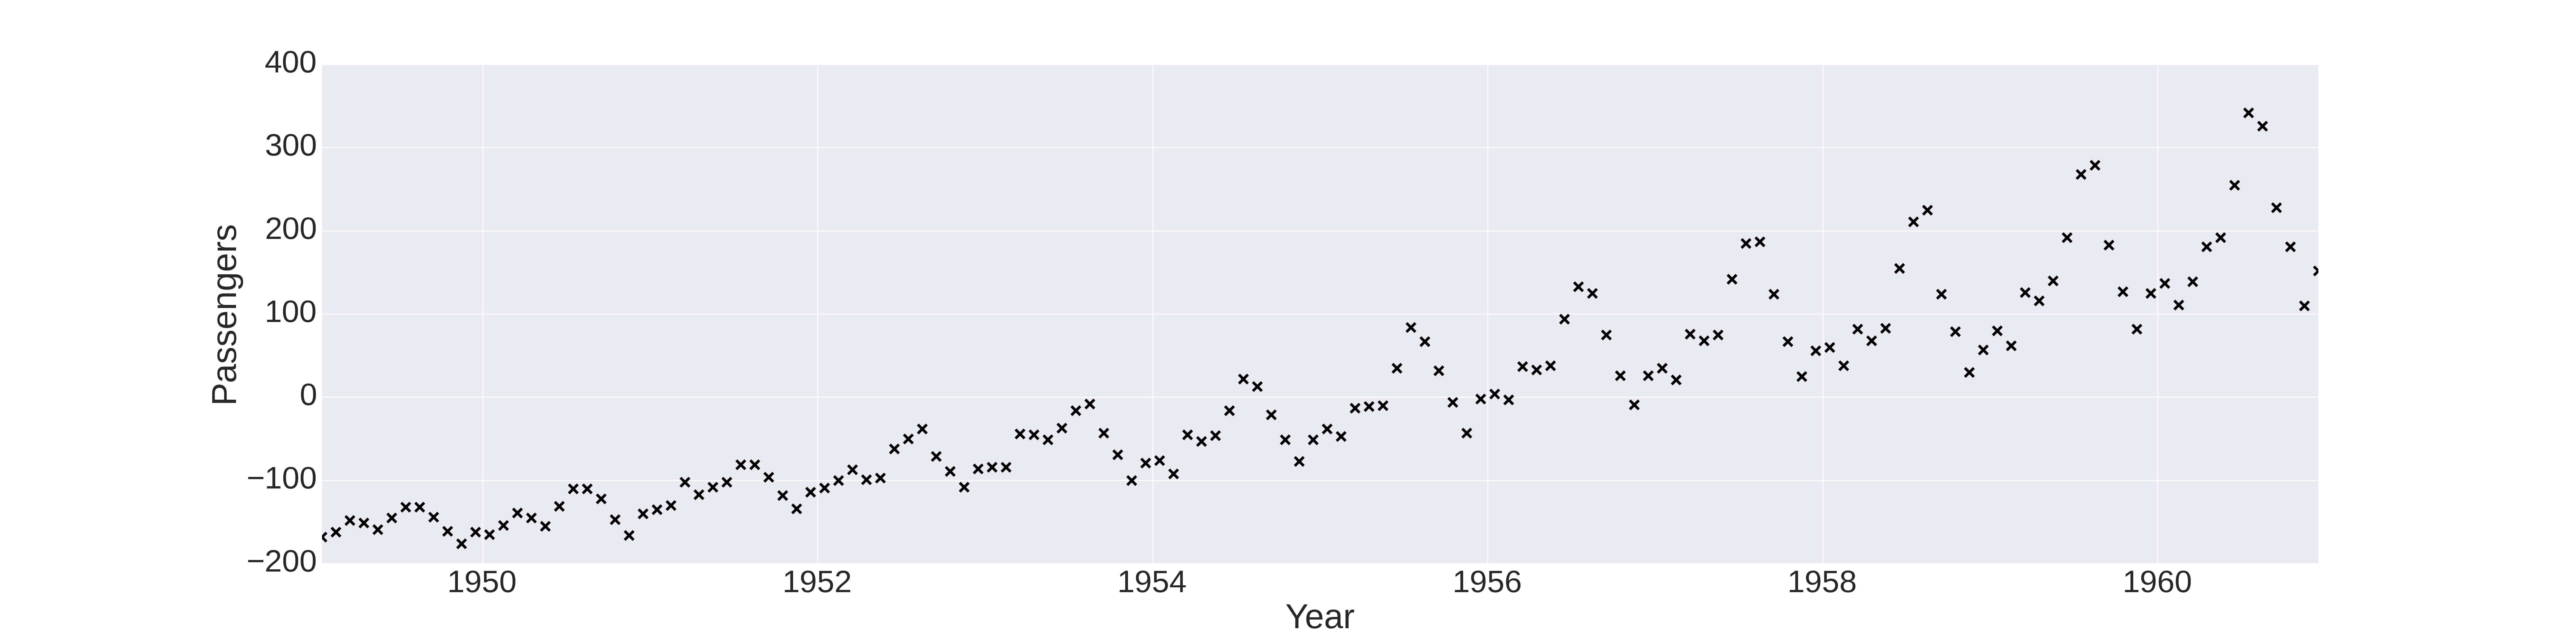
\includegraphics[width=\linewidth]{rawx.png}\\
\includegraphics[width=\linewidth]{priorx.png}\\
\includegraphics[width=\linewidth]{posteriorx.png}
\captionof{figure}{\color{DarkSlateGray} Top: raw data, monthly airline passengers. Middle, prior on functions. Bottom, posterior.}
\end{center}

 
\vfill
\columnbreak
%----------------------------------------------------------------------------------------
%	Bayesian Optimization
%----------------------------------------------------------------------------------------
\section*{Bayesian Optimization}
\subsection*{Thompson Sampling for Homogeneous Sequential Markov Decision Processes}

\noindent Two phases, each takes one line of code:
\begin{enumerate}
  \item Sample a context $V_\emu \sim P(V_\emu)$ using a Metropolis--Hastings sampler.
  \item Probe the point $x_\rmnext = \argmax_x V_\emu(x)$.
\end{enumerate}
\vspace{1cm}

\begin{minipage}{\linewidth}
\begin{lstlisting}[frame=single,label=alg:structureVent,mathescape]
assume sf = tag('hyper, log(uniform_continuous(0, 10)))
assume l = tag('hyper, log(uniform_continuous(0, 10)))
assume se = make_squaredexp(sf, l)
assume blackbox_f = get_bayesopt_blackbox()
assume compute_and_emu = gpmem(blackbox_f, se)

define get_uniform_candidate = proc(prev_xs) {
    uniform_continuous(-20, 20)
}

define mc_argmax = proc(f, prev_xs) {
    // Monte Carlo estimator for the argmax of f.
    run(do(
        candidate_xs <- mapv(proc(i) { get_uniform_candidate(prev_xs) },
                             linspace(0, 19, 20)),
        candidate_ys <- mapv(f, candidate_xs),
        lookup(candidate_xs, argmax_of_array(candidate_ys))))
}

define emulator_point_sample = proc(x) {
    run(sample(lookup(
        second(compute_and_emu)(array(x)),
        0)))
}

infer repeat(15, do(pass,
      // Phase 2: Call f_compute on the next probe point
      predict first(compute_and_emu)(
                  mc_argmax(emulator_point_sample, '_)),
      // Phase 1: Hyperparameter inference
      mh('hyper, one, 50)))
\end{lstlisting}
\end{minipage}
      
%Bayesian Optimization with Thompson sampling providing:
%\begin{itemize}
% \item  the ability to search over a broader space of contexts than the parametric families that are typically used;
% \item parsimony of the resulting probabilistic program.
%\end{itemize}

\subsection*{Results}
\begin{center}
  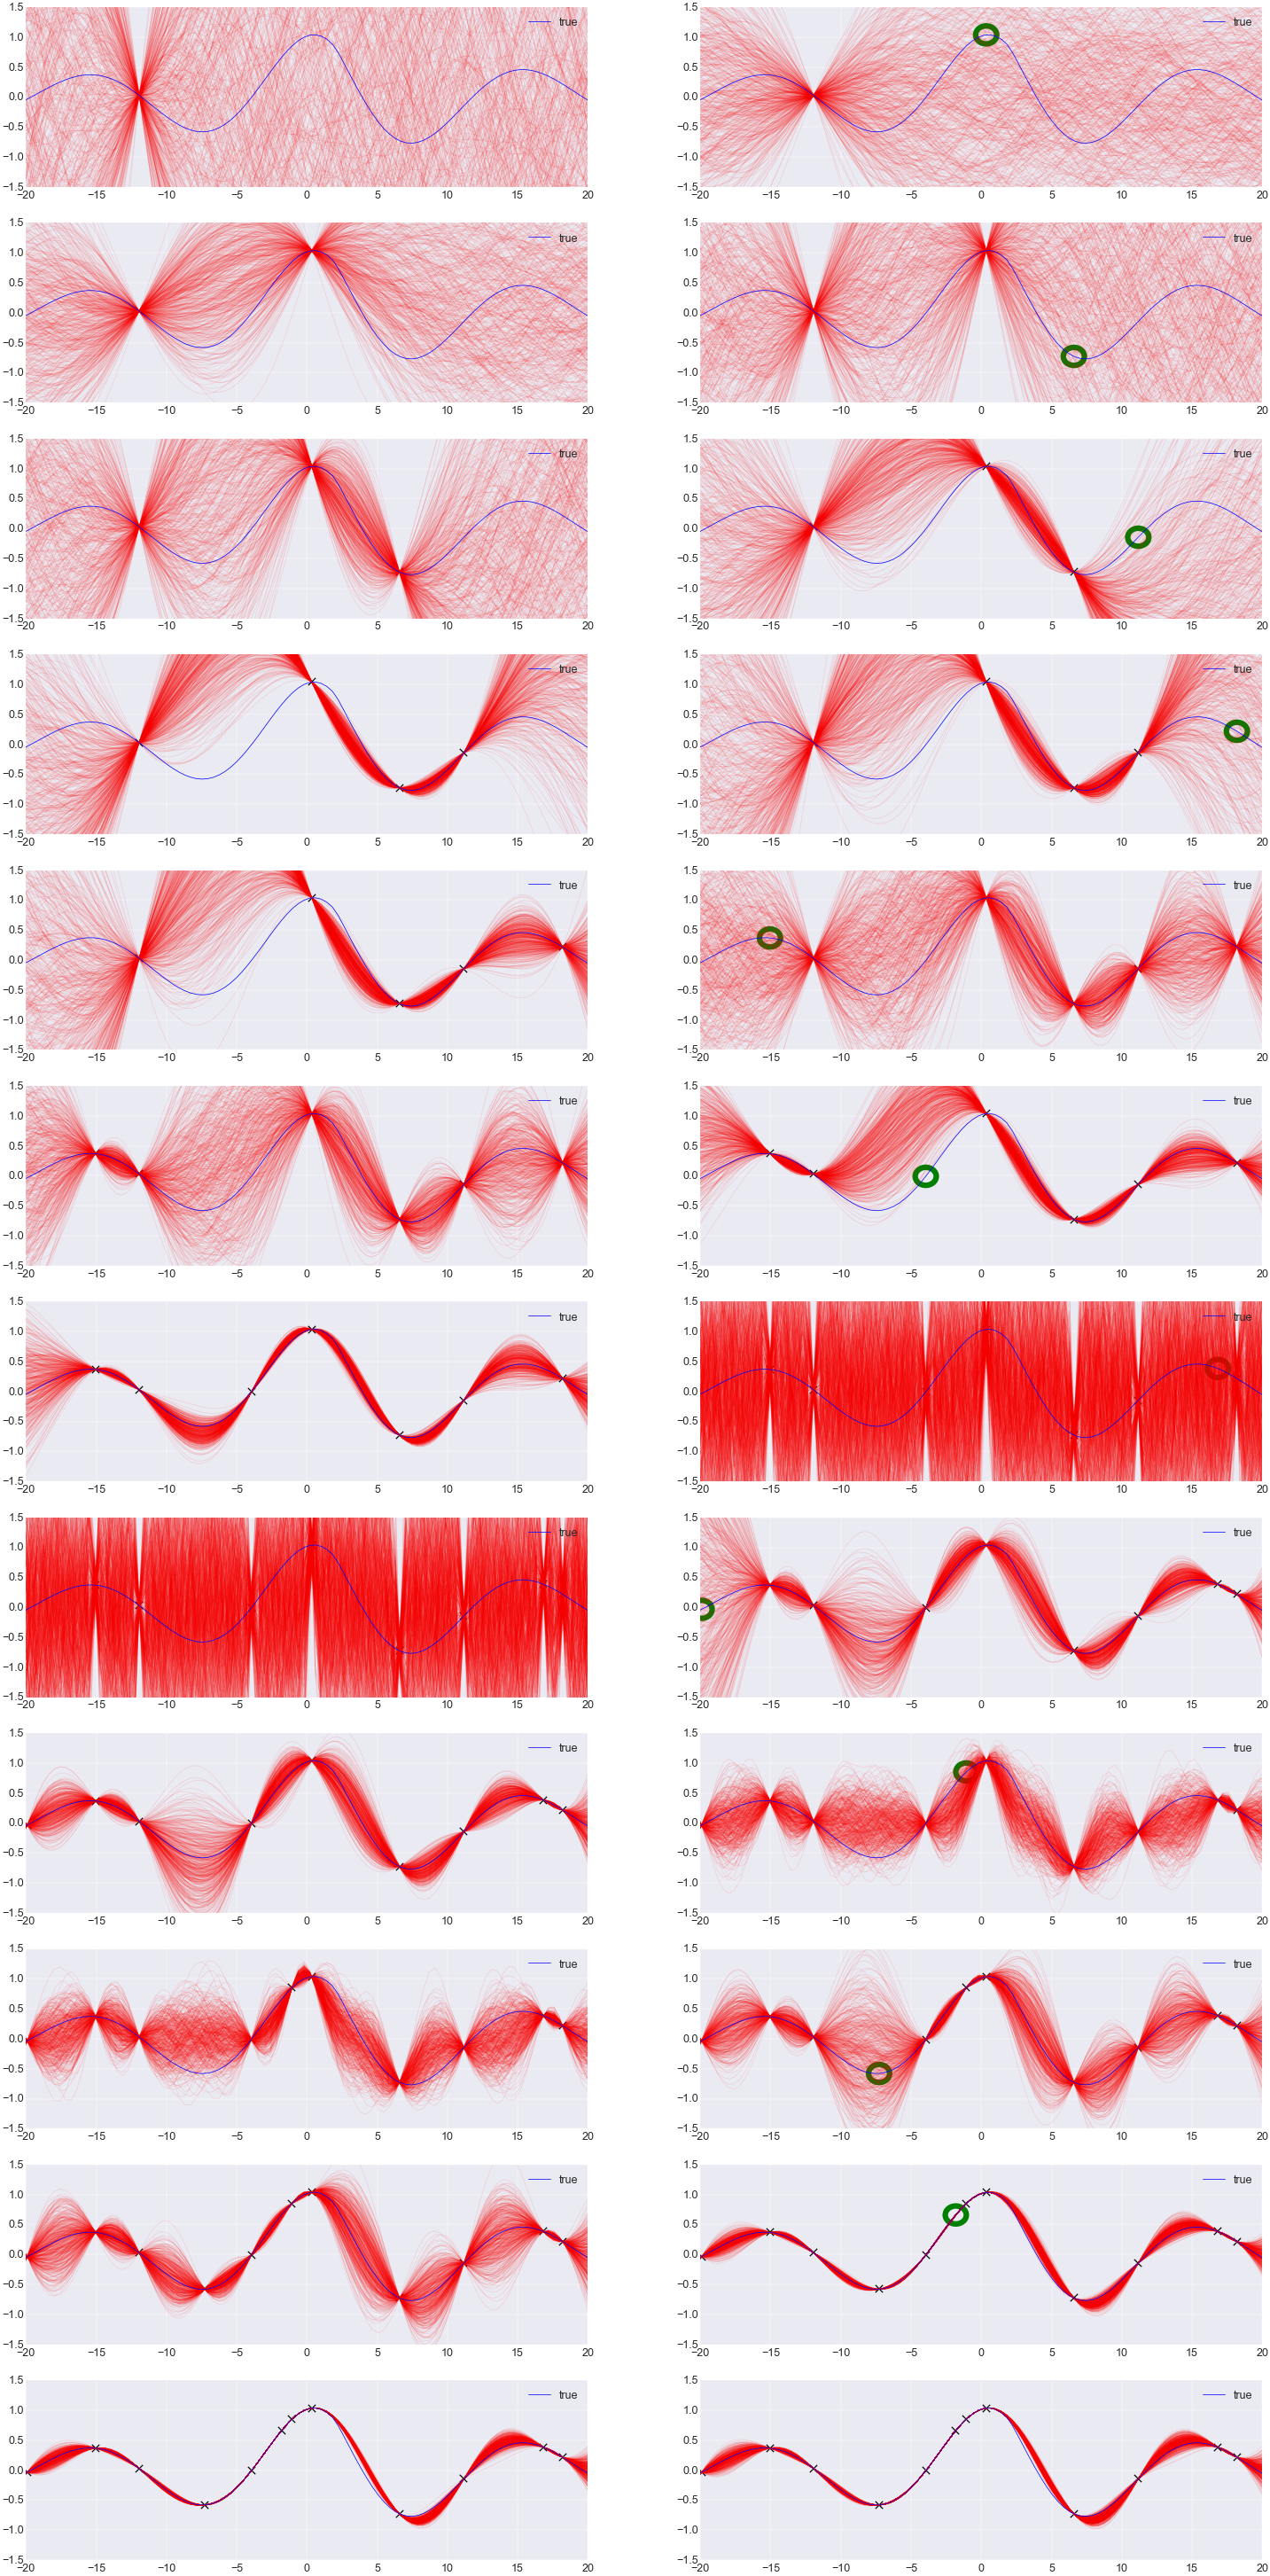
\includegraphics[width=20cm]{BayesOpt_gpmem_sequence.png}
\end{center}

\begin{itemize}
  \item Blue: Unknown true value function $V$
  \item Red: Current state of our statistical emulator $V_\emu$, conditioned on previously probed values of $V$
  \item Green: Next chosen probe point $x_\rmnext$
  \item Left: before hyperparameter inference; right: after hyperparameter inference
\end{itemize}
Probes tend to happen at points either where the value of $V_\emu$ is high, or where $V_\emu$ has high uncertainty.

     
     
%
%\begin{center}\vspace{1cm}
%\captionof{figure}{\color{DarkSlateGray} } \label{fig:bayesopt-sequence}
%\end{center}

   



%\section*{Conclusions}
%{\tt gpmem} is a generalization of a number of GP\newline related models and can be applied to:
%\begin{itemize}
%\setlength{\itemindent}{1cm}
%\item Hierarchical Bayesian GP
%\item Kernel Structure Learning
%\item Bayesian Optimization
%\end{itemize}

\color{DarkSlateGray} % Set the color back to DarkSlateGray for the rest of the content

%----------------------------------------------------------------------------------------
%	FORTHCOMING RESEARCH
%----------------------------------------------------------------------------------------

%\section*{Forthcoming Research}

%Vivamus molestie, risus tempor vehicula mattis, libero arcu volutpat purus, sed blandit sem nibh eget turpis. Maecenas rutrum dui %blandit lorem vulputate gravida. Praesent venenatis mi vel lorem tempor at varius diam sagittis. Nam eu leo id turpis interdum %luctus a sed augue. Nam tellus.

 %----------------------------------------------------------------------------------------
%	REFERENCES
%----------------------------------------------------------------------------------------
\small

\bibliographystyle{plain} % Plain referencing style
\bibliography{June2015} % Use the example bibliography file sample.bib

%----------------------------------------------------------------------------------------
%	ACKNOWLEDGEMENTS
%----------------------------------------------------------------------------------------

%\section*{Acknowledgements}


%----------------------------------------------------------------------------------------

\end{multicols}
\end{document}
